\subsection{Elektronik}

\author{Ervin Mazlagi\'c}

\begin{frame}
	\frametitle{Übersicht\hfill{}\footnotesize \group}
	\framesubtitle{Aufgaben \& Komponenten}
	\begin{columns}
		\begin{column}{0.5\textwidth}
			\begin{block}{Aufgaben}
				\begin{itemize}
					\item Energieversorgung
					\item Kommunikation mit Peripherie
					\item Ansteuerung der Peripherie
					\item Parametrierung der Maschine
				\end{itemize}
			\end{block}
		\end{column}
		\begin{column}{0.5\textwidth}
		\begin{figure}
			\begin{tikzpicture}[node distance=1.5cm]
				\footnotesize
				\node (pwr) [power] {PWR};
				\node (dc) [driver, below of=pwr] {DC};
				\node (bldc) [driver, below of=dc] {BLDC};
				\node (stp) [driver, below of=bldc] {STP};
				\node (mot1) [power, right of=dc] {MOT};
				\node (mot2) [power, right of=bldc] {MOT};
				\node (mot3) [power, right of=stp] {MOT};
				\node (frdm) [logic, left of=pwr] {FRDM};
				\draw[red,thick] (pwr) -| (mot1);
				\draw[red, thick] (mot1) -- (mot2);
				\draw[red, thick] (mot2) -- (mot3);
				\draw[red, thick] (pwr) -- (dc);
				\draw[red, thick] (dc) -- (bldc);
				\draw[red, thick] (bldc) -- (stp);
				\draw[blue, thick, <->] (frdm) |- (dc);
				\draw[blue, thick, <->] (frdm) |- (bldc);
				\draw[blue, thick, <->] (frdm) |- (stp);
				\draw[green, thick, ->] (dc) -- (mot1);
				\draw[green, thick, ->] (bldc) -- (mot2);
				\draw[green, thick, ->] (stp) -- (mot3);
			\end{tikzpicture}
		\end{figure}
		\end{column}
	\end{columns}
\end{frame}

\subsubsection{Fachgruppe ET}
\begin{frame}
	\frametitle{Fachgruppe Elektrotechnik\hfill{}\footnotesize \group}
	\framesubtitle{Motivation \& Ziele}
	\begin{columns}
		\begin{column}{0.5\textwidth}
				\textit{``Denn es ist eines ausgezeichneten
					Mannes nicht würdig, wertvolle Stunden
					wie ein Sklave im Keller der einfachen
					Berechnungen zu verbringen''}
				~ \\ ~ \\
				\hfill{} -- Gottfired Wilhelm Leibniz \\
		\end{column}
		\pause
		\begin{column}{0.5\textwidth}
			\begin{block}{Ziele}
				\begin{itemize}
					\item Synergien nutzen
					\item Fachlicher Austausch
					\item Eigenentwicklungen
					\item OpenHardware
				\end{itemize}
			\end{block}
		\end{column}
	\end{columns}
\end{frame}

\begin{frame}
	\frametitle{Fachgruppe Elektrotechnik \hfill{} \footnotesize \group}
	\framesubtitle{Organisation \& Projekte}
	\begin{columns}
		\begin{column}{0.5\textwidth}
			\begin{block}{github.com/pren-et}
				\begin{itemize}
					\item 7 Contributors
					\item 6 PREN-Teams
					\item 7 Repositories
					\item 3 HW-Projekte
				\end{itemize}
			\end{block}
		\end{column}
		\begin{column}{0.5\textwidth}
			\begin{exampleblock}{Projekte}
				\begin{itemize}
					\item Motorentreiber für
						\begin{itemize}
							\item DC
							\item BLDC
							\item Stepper
						\end{itemize}
					\item Dokumentationen
				\end{itemize}
			\end{exampleblock}
		\end{column}
	\end{columns}
\end{frame}

\subsubsection{Motoren}
\begin{frame}
	\frametitle{Motoren\hfill{}\footnotesize \group}
	\framesubtitle{Schrittmotor (Stepper) für Turmausrichtung}
	\begin{columns}
		\begin{column}{0.5\textwidth}
			\begin{figure}
				\begin{tikzpicture}[node distance=1.5cm]
					\footnotesize
					\node (frdm) [logic] {FRDM};
					\node (l6480) [driver, below of=frdm] {L6480};
					\node (stp) [power, below of=l6480] {STP};
					\draw[blue, thick, <->] (frdm) -- node[anchor=east] {UART} ($ (frdm) + (0,1) $);
					\draw[blue, thick, <->] (frdm) -- node[anchor=east] {SPI} (l6480);
					\draw[green, thick, ->] (l6480) -- (stp);
				\end{tikzpicture}
			\end{figure}
		\end{column}
		\begin{column}{0.5\textwidth}
		\end{column}
	\end{columns}
\end{frame}

\begin{frame}
	\frametitle{Motoren\hfill{}\footnotesize \group}
	\framesubtitle{Synchronmotor (BLDC) für Ballwurf}
	\begin{columns}
		\begin{column}{0.5\textwidth}
			\begin{figure}
				\begin{tikzpicture}[node distance=1.5cm]
					\footnotesize
					\node (frdm) [logic] {FRDM};
					\node (drv) [driver, below of=frdm] {DRV};
					\node (bldc) [power, below of=drv] {BLDC};
					\draw[blue, thick, <->] (frdm) -- node[anchor=east] {UART} ($ (frdm) + (0,1) $);
					\draw[blue, thick, <->] (frdm) -- node[anchor=east] {SPI} (l6480);
					\draw[green, thick, ->] (drv) -- (bldc);
				\end{tikzpicture}
			\end{figure}
		\end{column}
		\begin{column}{0.5\textwidth}
		\end{column}
	\end{columns}

\end{frame}

\begin{frame}
	\frametitle{Motoren\hfill{}\footnotesize \group}
	\framesubtitle{Gleichstrommotor (DC) für Ballnachführung}
	\begin{columns}
		\begin{column}{0.5\textwidth}
			\begin{figure}
				\begin{tikzpicture}[node distance=1.5cm]
					\footnotesize
					\node (frdm) [logic] {FRDM};
					\node (a3941) [driver, below of=frdm] {A3941};
					\node (dc) [power, below of=a3941] {DC};
					\draw[blue, thick, <->] (frdm) -- node[anchor=east] {UART} ($ (frdm) + (0,1) $);
					\draw[blue, thick, <->] (frdm) -- node[anchor=east] {PWM} (a3941);
					\draw[green, thick, ->] (a3941) -- (dc);
				\end{tikzpicture}
			\end{figure}
		\end{column}
		\begin{column}{0.5\textwidth}
		\end{column}
	\end{columns}

\end{frame}

\subsubsection{Mikrocontroller}
\begin{frame}
	\frametitle{Mikrocontroller\hfill{}\footnotesize \group}
	\framesubtitle{Freedomboard FRDM-KL25Z}
	\begin{columns}
		\begin{column}{0.5\textwidth}
			\begin{figure}
				\centering
				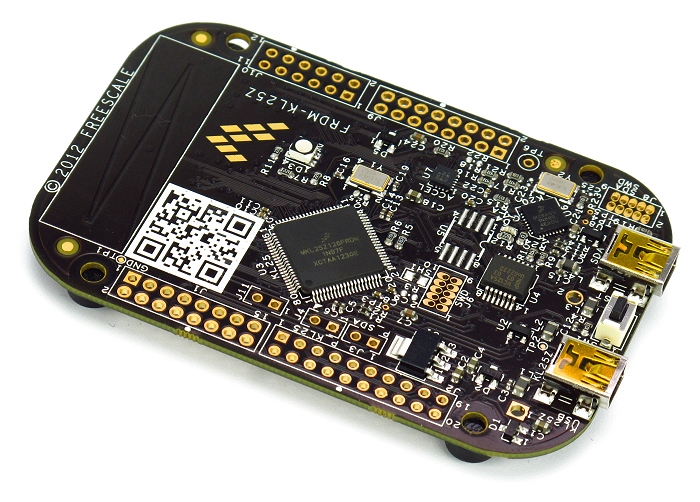
\includegraphics[width=1\textwidth]{../../fig/frdm-kl25z.jpg}
				\caption{FRDM-KL25Z}
			\end{figure}
		\end{column}
		\begin{column}{0.5\textwidth}
			\begin{itemize}
				\item LowLevel-Schnittstelle für
					\begin{itemize}
						\item Motoransteuerung
						\item Sensorik \& Messtechnik
						\item Busse (UART, SPI, I$^2$C)
					\end{itemize}
				\item Programmierung in C
				\item Kommunikation über UART
				\item Programmierung mit CW, KDS oder GCC möglich
			\end{itemize}
		\end{column}
	\end{columns}
\end{frame}

\subsubsection{Messtechnik}
\begin{frame}
	\frametitle{Messtechnik\hfill{}\footnotesize \group}
	\framesubtitle{Halleffekt-Schalter als Drehgeber}
\end{frame}
